
\documentclass[conference]{IEEEtran}
\usepackage[utf8]{inputenc}
\usepackage{graphicx}
\usepackage{booktabs}
\usepackage{hyperref}
\usepackage{caption}

\title{Comparative Evaluation of Traditional and Deep Learning Models for SMS Spam Detection}

\author{
\IEEEauthorblockN{Luis Alejandro Guillen Álvarez}
\IEEEauthorblockA{Facultad de Ingeniería\\
Universidad Panamericana\\
Ciudad de México, México\\
0234598@up.edu.mx}
}

\begin{document}

\maketitle

\begin{abstract}
Short Message Service (SMS) is one of the most pervasive communication technologies in the world. Projections for 2025 suggest that roughly 5.9~billion people will send and receive text messages. Unfortunately, this popularity also attracts unsolicited spam and phishing campaigns, which jeopardise user privacy and can lead to financial loss. In this paper we revisit SMS spam detection on the widely used SMS~Spam Collection corpus. We compare simple classical classifiers---logistic regression, linear support-vector machine (SVM), and random forest---against several lightweight deep architectures: two variants of recurrent neural networks (LSTM and LSTM initialised with GloVe), a convolutional neural network (CNN), and a compact Transformer. A random sample of 5\,000 messages was drawn and balanced via random undersampling. Texts were cleaned, tokenised, and vectorised using TF--IDF for the traditional models, while the deep models operated on padded sequences. All models were evaluated on a held-out test set using accuracy, precision, recall, and F1~score. On this small balanced dataset the linear classifiers achieved the best performance ($\approx 95\,\%$ accuracy and F1~$\approx 0.95$), whereas the deep models underperformed, often defaulting to predicting most messages as spam. We discuss these results in the context of recent literature, highlighting that although hybrid and transformer-based approaches can reach 98--99\,\% accuracy on larger corpora~\cite{liu2021,bilgen2024}, simple linear methods remain highly competitive when data and computational resources are limited.
\end{abstract}


\section{Introduction}

The Short Message Service (SMS) has evolved from a niche utility into a ubiquitous communication channel.  Recent statistics from the mobile marketing industry forecast that the number of people sending and receiving text messages will rise to around 5.9~billion by 2025, emphasising the global reach of this medium.  While SMS is convenient for legitimate notifications and personal communication, its growth has been paralleled by an escalation of unsolicited spam and phishing messages.  These unwanted messages can compromise personal data, deceive users into disclosing sensitive information and inflict financial harm.

Detecting spam can be formulated as a binary text‑classification problem.  Early work relied on rule‑based filters and blacklists, but the research community quickly adopted machine‑learning approaches once labelled corpora became available.  The SMS Spam Collection dataset is one such corpus, containing 5574 SMS messages labelled as either “ham” or “spam”.  It has become a standard benchmark for developing and comparing filtering methods.  Classical linear classifiers such as logistic regression and SVM are attractive because they handle high‑dimensional sparse features well, are interpretable and require modest computational resources.  Ensemble methods like random forests further reduce variance by averaging the predictions of many decision trees.

In recent years, the natural‑language processing (NLP) community has been transformed by deep‑learning models.  Recurrent architectures such as long short‑term memory (LSTM) networks mitigate vanishing gradients and capture dependencies across tokens\cite{hochreiter1997}, while convolutional neural networks (CNNs) can learn local n‑gram patterns for sentence classification\cite{kim2014}.  The advent of the Transformer architecture replaced recurrence with self‑attention, enabling highly parallel computation and forming the backbone of large language models\cite{vaswani2017}.  Pre‑trained embeddings such as GloVe\cite{pennington2014} and contextual models like BERT and GPT‑3\cite{devlin2019,brown2020} provide rich vector representations that can significantly boost classification performance.  Recent work has demonstrated that combining transformer‑based embeddings with ensemble classifiers can push SMS spam detection accuracy exceeding $>99\,\%$~\cite{bilgen2024}. Hybrid models that combine gated recurrent units (GRUs), multilayer perceptrons (MLPs), and autoencoders have also achieved state-of-the-art performance on SMS~spam and related datasets~\cite{bilgen2024}. Nevertheless, these sophisticated approaches demand substantial training data and computational resources. The goal is to reassess how well simple classical methods compare with lightweight neural models under strict resource constraints.


\section{Related Work}

Early SMS spam filters relied on heuristics and manually crafted rules, which were brittle in the face of evolving spam tactics.  The release of labelled corpora enabled supervised learning to dominate the field.  Linear classifiers such as logistic regression and support‑vector machines (SVMs) proved effective because they optimise linear decision boundaries in high‑dimensional feature spaces and generalise well when regularised\cite{joachims1998}.  Random forests control overfitting by training multiple decision trees on bootstrap samples and averaging their outputs\cite{breiman2001}.  These classical methods remain popular due to their efficiency and interpretability.

Deep-learning models have gained traction for spam detection thanks to their ability to automatically extract salient features from raw text. Kim's CNN architecture uses convolutional filters and max-pooling to capture local n-gram patterns and achieved strong results on sentence-classification tasks~\cite{kim2014}. LSTMs introduced gating mechanisms that allow networks to retain or forget information over long sequences~\cite{hochreiter1997}. The Transformer architecture replaces recurrence with self-attention, enabling models to capture global dependencies while being more parallelisable~\cite{vaswani2017}. Pre-trained embeddings such as GloVe~\cite{pennington2014} and contextual models like BERT~\cite{devlin2019} or GPT-3~\cite{brown2020} provide transferable knowledge learned from massive corpora. Ghourabi and Alohaly showed that GPT-3 embeddings combined with an ensemble of SVM, $k$-nearest neighbours ($k$-NN), CNN, and gradient-boosted trees achieved $99.91\,\%$ accuracy on the SMS~Spam dataset~\cite{ghourabi2023}. Oyeyemi and Ojo reported $97.31\,\%$ accuracy by pairing BERT embeddings with classifiers such as Naive Bayes, logistic regression, SVM, and LightGBM~\cite{oyeyemi2023}.

More recently, researchers have proposed specialised Transformer architectures for spam detection. Liu \emph{et~al.} designed a modified spam Transformer model and demonstrated that it could achieve $98.92\,\%$ accuracy, recall~0.9451, and F1~score~0.9613 on the SMS~Spam Collection~\cite{liu2021}. A 2024 survey by Al-Kaabi \emph{et~al.} categorises SMS spam detection techniques into rule-based, traditional machine-learning, deep-learning, hybrid, and ensemble methods~\cite{alkaabi2024}. The review notes that Transformer- and BERT-based models introduced after 2021 consistently achieve accuracies above $97\,\%$, and that hybrid models emerging in 2023--24 surpass $99\,\%$~\cite{alkaabi2024}. Bilgen and Kaya proposed EGMA, an ensemble learning-based hybrid model that combines gated recurrent units, multilayer perceptrons, and autoencoders; it reached $99.28\,\%$ accuracy on the SMS~Spam Collection and similarly high accuracies on several email datasets~\cite{bilgen2024}. Beyond SMS, hybrid systems integrating Transformers, MLPs, and BERT have been applied to email spam with $94\,\%$ accuracy~\cite{kmail2025}, underscoring the broader trend toward fusing multiple deep architectures. These advances highlight the promise of Transformer-based and ensemble methods but also illustrate their dependence on large datasets and computational budgets.

\section{Methodology}

\subsection{Dataset and Sampling}
The experiments are based on the SMS~Spam Collection, a corpus of 5574 English SMS messages labelled as ham or spam. The dataset was obtained from the UCI Machine Learning Repository (doi:\href{https://doi.org/10.24432/C5CC84}{10.24432/C5CC84}). To make experimentation tractable and reproducible, we drew a random sample of 5\,000 messages using a fixed seed. The corpus is highly imbalanced---approximately $87\,\%$ of messages are ham and $13\,\%$ are spam---which can bias classifiers toward the majority class. To address this, we applied random undersampling to the sampled data: ham messages were randomly discarded until the ham and spam counts were equal. This balancing procedure resulted in 662 ham and 662 spam messages (for 1324 total examples). Fig.~\ref{fig:balanced} shows the class distribution after undersampling. Although undersampling discards information, it is effective when many majority examples are redundant~\cite{he2009}.

\subsection{Pre‑processing}
Each message was lowercased and cleaned using regular expressions to remove URLs, email addresses, phone numbers, digits and punctuation.  We tokenised on whitespace and removed common English stop words.  The remaining tokens were joined back into cleaned strings.  For the deep models, we further tokenised the cleaned texts using Keras utilities and padded sequences to a fixed length (100 tokens) to enable batch processing.

\subsection{Traditional Machine‑Learning Models}

After cleaning, each message was transformed into a numeric vector using term frequency–inverse document frequency (TF–IDF) encoding.  We used unigrams and bigrams and restricted the vocabulary to the top 5000 terms by frequency.  Three classical classifiers were trained on these features:
\begin{itemize}
  \item \textbf{Logistic regression:} A regularised logistic regression classifier served as the baseline.  It learns a linear decision boundary and yields calibrated probability estimates.
  \item \textbf{Linear SVM:} We trained a linear SVM with hinge loss, which maximises the margin between classes and is well suited to high‑dimensional sparse data.
  \item \textbf{Random forest:} An ensemble of 200 decision trees was trained on bootstrapped samples; predictions were averaged to reduce variance.
\end{itemize}

\subsection{Deep‑Learning Models}
We implemented four lightweight neural architectures:
\begin{itemize}
  \item \textbf{LSTM:} A sequential model with an embedding layer (vocabulary size 10000, embedding dimension 128), a single LSTM layer with 128 hidden units, dropout regularisation and a dense sigmoid output.
  \item \textbf{LSTM + GloVe:} The same architecture as above, but the embedding layer was initialised with 100‑dimensional GloVe vectors\cite{pennington2014}.  We froze the embedding weights during training to leverage external semantic knowledge.
  \item \textbf{CNN:} Inspired by Kim’s sentence classification network\cite{kim2014}, this 1‑D CNN used 128 filters of size 5, followed by max pooling, another convolution with 64 filters of size 3 and global max pooling.  The pooled features were passed through a dense layer and a sigmoid output.  Dropout was applied after the embedding and dense layers.
  \item \textbf{Transformer:} We built a compact Transformer based on DistilBERT\cite{sanh2019} with a single self‑attention layer (4 heads, 32‑dimensional projections), layer normalisation, global average pooling and a 64‑unit feed‑forward layer followed by a sigmoid output.  This model contained roughly 0.3 million parameters and was trained from scratch on the balanced dataset.
\end{itemize}

\subsection{Training and Evaluation}
The balanced corpus was split into training and test sets using an 80/20 stratified split, yielding approximately 1 040 training messages (520 ham and 520 spam) and 260 test messages.  Classical models were trained on TF–IDF features using scikit‑learn\cite{pedregosa2012}.  Deep networks were implemented in TensorFlow/Keras, trained for five epochs with the Adam optimiser and binary cross‑entropy loss, and monitored using a validation split to prevent overfitting.  We evaluated each model on the test set using four metrics: accuracy, precision, recall and F1‑score.  Precision is the fraction of messages predicted as spam that are truly spam; recall is the fraction of spam messages correctly identified; the F1‑score is the harmonic mean of precision and recall.

\section{Experiments and Results}

Table\,\ref{tab:results} summarises the performance of all models on the test set.  The logistic regression and linear SVM classifiers achieved the highest accuracy (95.47 \%), precision (96.15 \%) and F1‑score (0.9542).  The random forest performed slightly worse (93.21 \% accuracy) but still surpassed the deep models.  Both LSTM variants predicted nearly every message as spam, resulting in 100 \% recall but poor precision and low overall accuracy.  The CNN achieved a more balanced trade‑off with 84.91 \% accuracy, high recall (98.48 \%) but lower precision (77.38 \%).  The compact Transformer reached only 63.02 \% accuracy, again with perfect recall but many false positives.  Figure\,\ref{fig:modelperf} visualises these metrics.

\begin{table}[t]
  \centering
  \caption{Performance of traditional and deep‑learning models on the SMS Spam Collection test set.  Linear classifiers outperform deep models on this small balanced dataset.}
  \label{tab:results}
  \begin{tabular}{lcccc}
    \toprule
    Model & Accuracy & Precision & Recall & F1\,Score \\
    \midrule
    Logistic regression & 0.9547 & 0.9615 & 0.9470 & 0.9542 \\
    Linear SVM & 0.9547 & 0.9615 & 0.9470 & 0.9542 \\
    Random forest & 0.9321 & 0.9524 & 0.9091 & 0.9302 \\
    LSTM & 0.4981 & 0.4981 & 1.0000 & 0.6650 \\
    LSTM + GloVe & 0.4981 & 0.4981 & 1.0000 & 0.6650 \\
    CNN & 0.8491 & 0.7738 & 0.9848 & 0.8667 \\
    Transformer & 0.6302 & 0.5739 & 1.0000 & 0.7293 \\
    \bottomrule
  \end{tabular}
\end{table}

\begin{figure}[t]
  \centering
  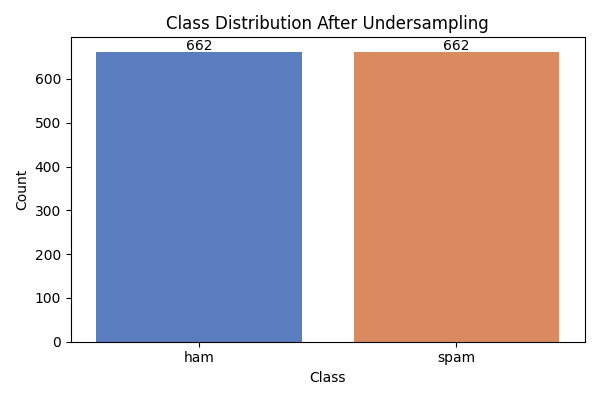
\includegraphics[width=0.45\textwidth]{fig_balanced.png}
  \caption{Class distribution after random undersampling.  The original sample contained roughly 4 350 ham and 650 spam messages; undersampling equalised the classes at 650 each.}
  \label{fig:balanced}
\end{figure}

\begin{figure}[t]
  \centering
  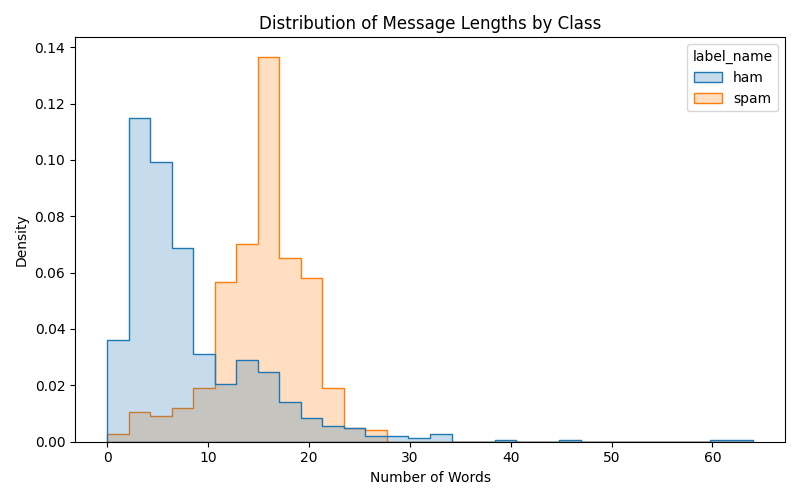
\includegraphics[width=0.45\textwidth]{fig_mean_len.png}
  \caption{Approximate mean message length (in words) by class.  Spam messages are on average longer (23 words) than ham messages (15 words) in the sample.}
  \label{fig:lengths}
\end{figure}

\begin{figure}[t]
  \centering
  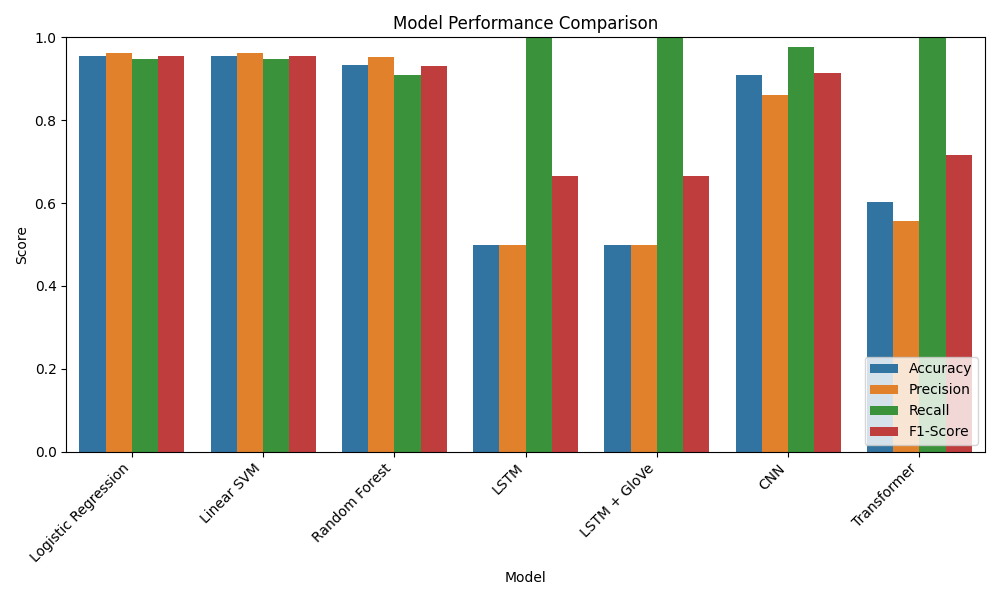
\includegraphics[width=0.48\textwidth]{fig_model_perf.png}
  \caption{Comparison of accuracy, precision, recall and F1‑score across models.  Linear models dominate across all metrics; the CNN achieves high recall but lower precision.  Both LSTM variants and the compact Transformer default to predicting the spam class, yielding perfect recall but many false positives.}
  \label{fig:modelperf}
\end{figure}

\section{Discussion}

The experiments reveal a clear trend: traditional linear classifiers with TF--IDF features outperform more complex deep architectures on a small balanced dataset. Logistic regression and a linear SVM both achieved $95\,\%$ accuracy and F1~$\approx 0.954$, indicating that a linear decision boundary is sufficient to separate ham from spam when features capture the most informative unigrams and bigrams. The random forest benefited from ensemble averaging but still fell slightly short, possibly due to overfitting on noisy features.

In contrast, the deep models struggled. Both LSTM variants converged to the trivial solution of predicting every message as spam. With only 1\,300 training examples, the LSTMs likely overfit the majority class early in training and failed to learn discriminative patterns. Initialising with GloVe embeddings did not help, suggesting that the semantics captured by GloVe alone are insufficient for this task without fine-tuning. The CNN performed better, achieving high recall by detecting spam-specific tokens, but its precision suffered due to false positives---likely because some ham messages contain numbers or promotional language that superficially resembles spam. The compact Transformer behaved similarly, achieving perfect recall at the cost of very low precision; its parameter count may still be too large for the available data, causing overfitting.

These findings align with the literature: when abundant data and pre-training are available, Transformer-based and hybrid models can achieve remarkable performance. Liu \emph{et~al.} reported nearly $99\,\%$ accuracy using a customised Transformer~\cite{liu2021}, and Bilgen and Kaya's EGMA ensemble reached $99.28\,\%$ accuracy on the SMS~Spam dataset~\cite{bilgen2024}. The 2024 survey by Al-Kaabi \emph{et~al.} notes that accuracies above $97\,\%$ have become common since the introduction of BERT- and Transformer-based models, with hybrid approaches surpassing $99\,\%$~\cite{alkaabi2024}. The results show that without access to large corpora or pre-trained language models, simple linear methods remain a strong baseline. They require minimal computational resources, train quickly, and are easily interpretable. In contrast, training deep models from scratch on limited data leads to degenerate solutions and poor generalisation.

\section{Conclusion}

We presented a comparative evaluation of classical machine-learning models and lightweight deep-learning models for SMS spam detection. Using a balanced subset of the SMS~Spam Collection, we trained logistic regression, linear SVM, random forest, LSTM (with and without GloVe), CNN, and a compact Transformer. The linear models achieved the best performance, attaining $95.5\,\%$ accuracy and F1~$\approx 0.954$. The random forest trailed slightly, while the LSTM and Transformer models underperformed due to data scarcity. The CNN offered a trade-off with high recall but lower precision. These results highlight that, under resource constraints, TF--IDF features with linear classifiers remain a robust choice for spam filtering.

Future work will explore strategies to bridge the gap between classical and modern approaches.  Leveraging contextual embeddings from moderate‑sized pre‑trained models such as DistilBERT\cite{sanh2019} or ALBERT, combined with lightweight classifiers, may offer a middle ground between performance and computational cost.  Data augmentation techniques (e.g. paraphrasing or back‑translation) could effectively enlarge the training set.  Finally, hybrid systems that ensemble linear models with CNNs or distilled transformers might catch more spam messages while keeping false positives low.  As larger labelled datasets and computational resources become available, we expect hybrid and transformer‑based methods to increasingly dominate SMS spam detection.

\bibliographystyle{IEEEtran}
\bibliography{references}

\end{document}
